\documentclass[12pt]{report}

\usepackage[left=0.75in, right=0.75in, top=0.75in, bottom=0.75in]{geometry}
\setlength\parindent{0pt}

\usepackage{graphicx, amsmath,anonchap,tabularx,multicol}
\usepackage{wrapfig}
\usepackage{vwcol}

\usepackage{enumitem}
\setlist{noitemsep}
\setlist{nolistsep}

\newenvironment{boxe}
    {\begin{center}
    \begin{tabular}{|p{0.9\textwidth}|}
    \hline\\
    }
    { 
    \\\\\hline
    \end{tabular} 
    \end{center}
    }

\begin{document}
\begin{tabular*}{\textwidth}{@{\extracolsep{\fill}}l l}
\textbf{Properties and Applications of Definite Integrals} \\
MATH 160\\
%\textbf{Due Friday, 10/22/18} & MATH 157\\
\hline\hline
\end{tabular*}\\
\begin{boxe}
For a continuous function $f(x)$ on the interval $[a,b]$ the \textbf{Definite Integral} is defined by the limit of a Riemann sum
$${\int_{a}^{b}f(x)\,dx=\lim_{n\rightarrow \infty}}\left(\sum_{i=0}^{n-1}f(x_i)\Delta x\right)$$\\
Where $f(x)$ is called the \textit{integrand} and $a$ and $b$ are called the limits of integration.\\\\
The \textbf{units} of a definite integral can be found by multiplying the units of the integrand (the units of $f(x)$) with the units of $dx$, the variable the integral is with respect to (the variable of integration).\\\\

\textbf{The FUNdamental Theorem of Calculus:} If $f(t)$ is continuous on the interval $[a,b]$ and $\frac{d}{dt}[F(t)]=f(t)$ then
$$\int_{a}^{b}f(t)\,dt=\int_{a}^{b}F'(t)\,dt=F(b)-F(a)$$
This tells use that in order to compute a definite integral we need to find a function $F(t)$ whose derivative is equal to $f(t)$ (where $F(t)$ is called \textit{an} anti-derivative of $f(t)$).\\\\

An \textbf{Antiderivative} of a function $f(x)$ is a function $F(x)$ such that $\frac{d}{dx}[F(x)]=f(x)$.\\
\begin{quote}
\vspace{-.25in}
    The \textbf{Family of Antiderivatives} of a function $f(x)$ are all up-down translations of $F(x)$. This is denoted as $F(x)+C$ where $C$ is any constant.
    \vspace{-.29in}
\end{quote}
\end{boxe}

\subsection*{Interpreting Definite Integrals}
\begin{boxe}
    1) Definite Integrals compute \textbf{Total Net Change}. Integrals are one way we can undo derivatives: we can take quantities like velocity, rates of change, quantities that measure "how fast" somethings changes and get quantities that measure a total net change like displacement.
    Ex. The displacement of an object between $t=a$ and $t=b$ whose velocity is $v(t)$ can be computed with the definite integral $\displaystyle{\int_{a}^bv(t) dt}$.\\\\    

    \begin{minipage}{0.65\textwidth}
    2) Definite Integrals compute \textbf{Signed Area} between a curve and the $x$-axis. This means definite integrals measure the area between a curve and the $x$-axis with area above the $x$-axis being positive and area below being negative. To the right is an example of the signed area between a curves and the $x$-axis on the interval $[a,b]$. 
    \end{minipage}
    \hfill
    \begin{minipage}{0.2\textwidth}
    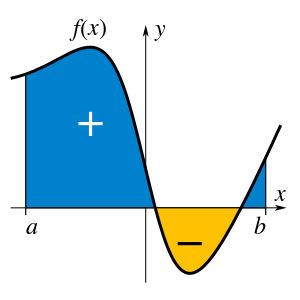
\includegraphics[scale=.3]{300px-Integral_example.svg.png}
    \end{minipage}
\end{boxe}

\subsection*{Properties of Definite Integrals}
\begin{boxe}
\textbf{Limits of Integration}:\\ Splitting: $\displaystyle{\int_{a}^{b}f(x)\,dx=\int_{a}^{c}f(x)\,dx+\int_{c}^{b}f(x)\,dx}$\\
Flipping : $\displaystyle{\int_{a}^{b}f(x)\,dx=-\int_{b}^{a}f(x)\,dx}$\\
\textbf{Constant Multiples}: $\displaystyle{\int_{a}^{b}cf(x)\,dx=c\int_{a}^{b}f(x)\,dx}$\\
\textbf{Adding Definite Integrals}: $\displaystyle{\int_{a}^{b}f(x)\pm g(x)\,dx=\int_{a}^{b}f(x)\,dx\pm \int_{a}^{b}g(x)\,dx}$\\
\textbf{Symmetry:}\\ 
If $f(x)$ is an \textbf{even function} (meaning $f(-x)=f(x)$) then $\displaystyle{\int_{-a}^{a}f(x)\,dx=2\int_{0}^{2}f(x)\,dx}$\\
If $f(x)$ is an \textbf{odd function} (meaning $f(-x)=-f(x)$) then $\displaystyle{\int_{-a}^{a}f(x)\,dx=0}$
\end{boxe}
\subsection*{Applications of Definite Integrals}
\begin{boxe}
\textbf{Area Between Curves}: If $f(x)\leq g(x)$ (meaning $g(x)$ is above $f(x)$) on the interval $[a,b]$ then the area between the curves $f$ and $g$ on the interval $[a,b]$ is $\displaystyle{\int_{a}^{b}g(x)-f(x)\,dx}$.\\
\begin{quote}
\vspace{-.25in}
    \textbf{CAUTION:} With curves that intersect: find all points of intersection in your interval and compute the area between the intersections separately.
\end{quote}

    \iffalse To the right is a visual example of the area enclosed by the curves $f(x)$ and $g(x)$ and the area \\
    \begin{wrapfigure}{r}{0.20\textwidth}
    \centering
    \includegraphics[width=0.20\textwidth]{areabetweencurve.png}
    \end{wrapfigure}
    \fi

\textbf{Average values}: The average value of a function $f(x)$ on the interval $[a,b]$ can be computed with the definite integral $\displaystyle{\frac{1}{b-a}\int_{a}^{b}f(x)\,dx}$
\end{boxe}



\end{document}
